\chapter{Lezione 1}
\label{chap:lezione_01} 

\begin{flushright}
\textit{Data: 01/10/2025}
\end{flushright}


\section{Introduzione al Corso}
Questo corso si propone di illustrare cosa cambia in alcuni modelli fondamentali, che magari abbiamo già incontrato, quando vengono resi più complessi. Essendo un corso di meccanica statistica, il nostro punto di partenza sarà il \textbf{modello di Ising}, che rivedremo e risolveremo di nuovo per introdurre tecniche non convenzionali come la fisica del disordine. Su questo modello base andremo poi a costruire modelli più complicati, introducendo elementi di disordine.

Affronteremo concetti come le transizioni di fase, la rottura spontanea di simmetria, la metastabilità e la rottura dell'ergodicità, analizzandoli separatamente, poiché nei modelli che studieremo questi fenomeni possono avvenire in momenti e per motivi diversi. Partendo dal modello di Ising, introdurremo il disordine passando al modello di "random field", per poi dedicare l'intera seconda metà del corso agli \textbf{spin glass}.

Il corso si concentrerà sugli aspetti tecnici; impareremo a fare i conti con il metodo delle repliche e il metodo della cavità. L'obiettivo finale è quello di essere in grado di risolvere i sistemi più complicati che oggi sappiamo trattare: i sistemi disordinati su grafi arbitrari (grafi random), che hanno innumerevoli applicazioni.


\section{Il Modello di Hopfield}

Il modello di Hopfield rappresenta un esempio affascinante di applicazione della meccanica statistica a un campo completamente diverso, quello delle neuroscienze. Il modello è stato introdotto da John Hopfield, un fisico che si è interessato ai processi cognitivi dal punto di vista biologico, nel tentativo di modellizzare il meccanismo di propagazione dell'informazione all'interno del cervello nel modo più semplice possibile.

\subsubsection{Modellizzazione del Neurone}
Il primo passo consiste nel semplificare al massimo il comportamento di un neurone. L'attività di un neurone è caratterizzata fondamentalmente da due stati: uno stato in cui è a riposo ("dormiente") e uno stato in cui si attiva e rilascia un potenziale d'azione ("spara"). Per modellizzare questo comportamento, discretizziamo il sistema sia nello spazio (considerando $N$ neuroni) sia nel tempo e associamo lo stato del neurone $i$ al tempo $t$ a una variabile di spin, $S_i^t$, che può assumere due valori. Per convenzione, usiamo i valori $\pm 1$:
\begin{equation}
S_i^t \in \{-1, 1\}
\end{equation}
dove $S_i^t = +1$ rappresenta lo stato in cui il neurone "spara" e $S_i^t = -1$ quello in cui "non spara".

\subsubsection{Dinamica della Rete}
Un neurone decide se sparare o meno in base ai segnali che riceve dagli altri neuroni a cui è connesso. In un modello a campo medio (fully connected), in cui ogni neurone interagisce con tutti gli altri, il segnale totale ricevuto dal neurone $i$ al tempo $t$ è dato dalla somma pesata degli stati di tutti gli altri neuroni:
\begin{equation}
\text{Segnale}_i^t = \sum_{j \neq i} J_{ij} S_j^t
\end{equation}
I termini $J_{ij}$ sono i \textbf{pesi sinaptici} e rappresentano l'intensità e la natura della connessione tra il neurone $j$ e il neurone $i$. Queste connessioni possono essere di due tipi:
\begin{itemize}
\item \textbf{Eccitatorie ($J_{ij} > 0$):} se il neurone $j$ spara, induce il neurone $i$ a sparare.
\item \textbf{Inibitorie ($J_{ij} < 0$):} se il neurone $j$ spara, induce il neurone $i$ a non sparare, depolarizzandolo.
\end{itemize}
La dinamica del sistema è definita da una semplice regola di aggiornamento. Lo stato del neurone $i$ al tempo successivo, $t+1$, è determinato dal segno del segnale totale che riceve. Se il segnale supera una soglia (che per semplicità poniamo a zero), il neurone sparerà; altrimenti, non sparerà. Matematicamente:

\begin{tcolorbox}[colback=yellow!30,  
                  colframe=yellow!50!orange,  
                  boxrule=0.8pt, 
                  arc=3pt,  
                  top=4pt, bottom=4pt, left=6pt, right=6pt,
                  enhanced,
                  sharp corners=south]
\begin{equation}
S_i^{t+1} = \text{sign}\left(\sum_{j \neq i} J_{ij} S_j^t\right)
\end{equation}
\end{tcolorbox}


Questa è una dinamica deterministica e parallela: dato uno stato iniziale della rete $S^0$, l'evoluzione del sistema è completamente definita.

\subsection{Memoria Associativa e Punti Fissi}
L'evoluzione di uno stato $S$ della rete può essere vista come una traiettoria nello spazio delle configurazioni: $S^0 \rightarrow S^1 \rightarrow S^2 \rightarrow \dots \rightarrow S^*$. 

Uno stato $S^*$ è un \textbf{punto fisso} della dinamica se, una volta raggiunto, il sistema non evolve più, ovvero viene mappato in se stesso dalla regola di aggiornamento.

Questo processo può essere interpretato, dal punto di vista neurofisiologico, come il \textbf{recupero di un ricordo}. Lo stato iniziale $S^0$ può essere pensato come l'input sensoriale che il cervello riceve . La successiva dinamica interna porta il sistema a convergere verso un punto fisso $S^*$, che rappresenta il concetto o il ricordo associato a quell'input. Questo è il motivo per cui il modello è detto di \textbf{memoria associativa}: stati iniziali diversi, purché sufficientemente simili a un ricordo immagazzinato, convergono allo stesso punto fisso.

\subsection{La Regola di Apprendimento di Hebb}
La domanda fondamentale è: come devono essere scelti i pesi sinaptici $J_{ij}$ affinché i punti fissi della dinamica corrispondano a specifici ricordi che vogliamo immagazzinare?. Le connessioni sinaptiche nel cervello non sono fisse, ma si alterano quando impariamo. Hopfield propose di utilizzare la \textbf{regola di Hebb}, un principio neuroscientifico secondo cui "neuroni che si attivano insieme, si collegano" (\textbf{neurons that fire together, wire together}).

Supponiamo di voler memorizzare $P$ "pattern" o ricordi, $\underline{\xi}^\mu$, con $\mu = 1, \dots, P$. Ogni pattern è un vettore di $N$ componenti, dove $N$ è il numero di neuroni (o spin), e $\xi_i^\mu \in \{-1, 1\}$. La regola di Hebb prescrive di definire i pesi sinaptici come segue:

\begin{tcolorbox}[colback=yellow!30,  
                  colframe=yellow!50!orange,  
                  boxrule=0.8pt, 
                  arc=3pt,  
                  top=4pt, bottom=4pt, left=6pt, right=6pt,
                  enhanced,
                  sharp corners=south]
\begin{equation}
J_{ij} = \frac{1}{N} \sum_{\mu=1}^{P} \xi_i^\mu \xi_j^\mu
\end{equation}
\end{tcolorbox}


Questa formula ha un'interpretazione biologica intuitiva: se, per un dato ricordo $\mu$, due neuroni $i$ e $j$ sono coerenti (cioè $\xi_i^\mu$ e $\xi_j^\mu$ hanno lo stesso segno), il loro contributo al peso $J_{ij}$ è positivo, rafforzando la loro connessione. Se invece sono incoerenti, il contributo è negativo, creando una connessione inibitoria. Questo processo può essere visto come il risultato di un \textbf{processo di apprendimento}: presentando ripetutamente i pattern alla rete, le connessioni sinaptiche si adattano per codificare queste memorie, \textbf{favorendo i neuroni coerenti}.

\subsection{Connessione con la Meccanica Statistica}
La dinamica di Hopfield ha una profonda connessione con la meccanica statistica. La regola di aggiornamento è equivalente a una dinamica a temperatura zero (gradient descent) che minimizza un'energia, o \textbf{Hamiltoniana}. Consideriamo un'Hamiltoniana della forma:
\begin{equation}
H = - \sum_{i<j} J_{ij} S_i S_j
\end{equation}
L'energia che coinvolge un singolo spin $S_i$ può essere scritta come:

\begin{equation}
H_i = -S_i \left( \sum_{j \neq i} J_{ij} S_j \right)
\end{equation}

La quantità tra parentesi è il \textbf{campo locale} sentito dallo spin $S_i$:

\begin{equation}
h_i = \sum_{j \neq i} J_{ij} S_j
\end{equation}

\begin{tcolorbox}[colback=yellow!30,  
                  colframe=yellow!50!orange,  
                  boxrule=0.8pt, 
                  arc=3pt,  
                  top=4pt, bottom=4pt, left=6pt, right=6pt,
                  enhanced,
                  sharp corners=south]

Per minimizzare l'energia, lo spin $S_i$ tenderà ad allinearsi con il suo campo locale, ovvero $S_i = \text{sign}(h_i)$. Questa è esattamente la dinamica di Hopfield.

Di conseguenza, \textbf{i punti fissi della dinamica corrispondono ai minimi locali dell'Hamiltoniana $H$}.
\end{tcolorbox}


Questa equivalenza permette di studiare le proprietà della rete, come la sua capacità di memorizzazione, utilizzando gli strumenti della meccanica statistica. Invece di analizzare la dinamica, si studiano le proprietà termodinamiche del sistema descritto da $H$ alla distribuzione di Gibbs-Boltzmann $P_{GB}(S) \propto e^{-\beta H}$, dove $\beta=1/T$.

\subsection{Diagramma di Fase del Modello di Hopfield}
Si studia il modello nel limite termodinamico ($N \rightarrow \infty$) e mantenendo costante il rapporto $\alpha = P/N$, detto \textbf{carico della rete}. Il diagramma di fase nel piano $(\alpha, T)$ rivela tre regioni principali:

\begin{figure}[h!]
\centering
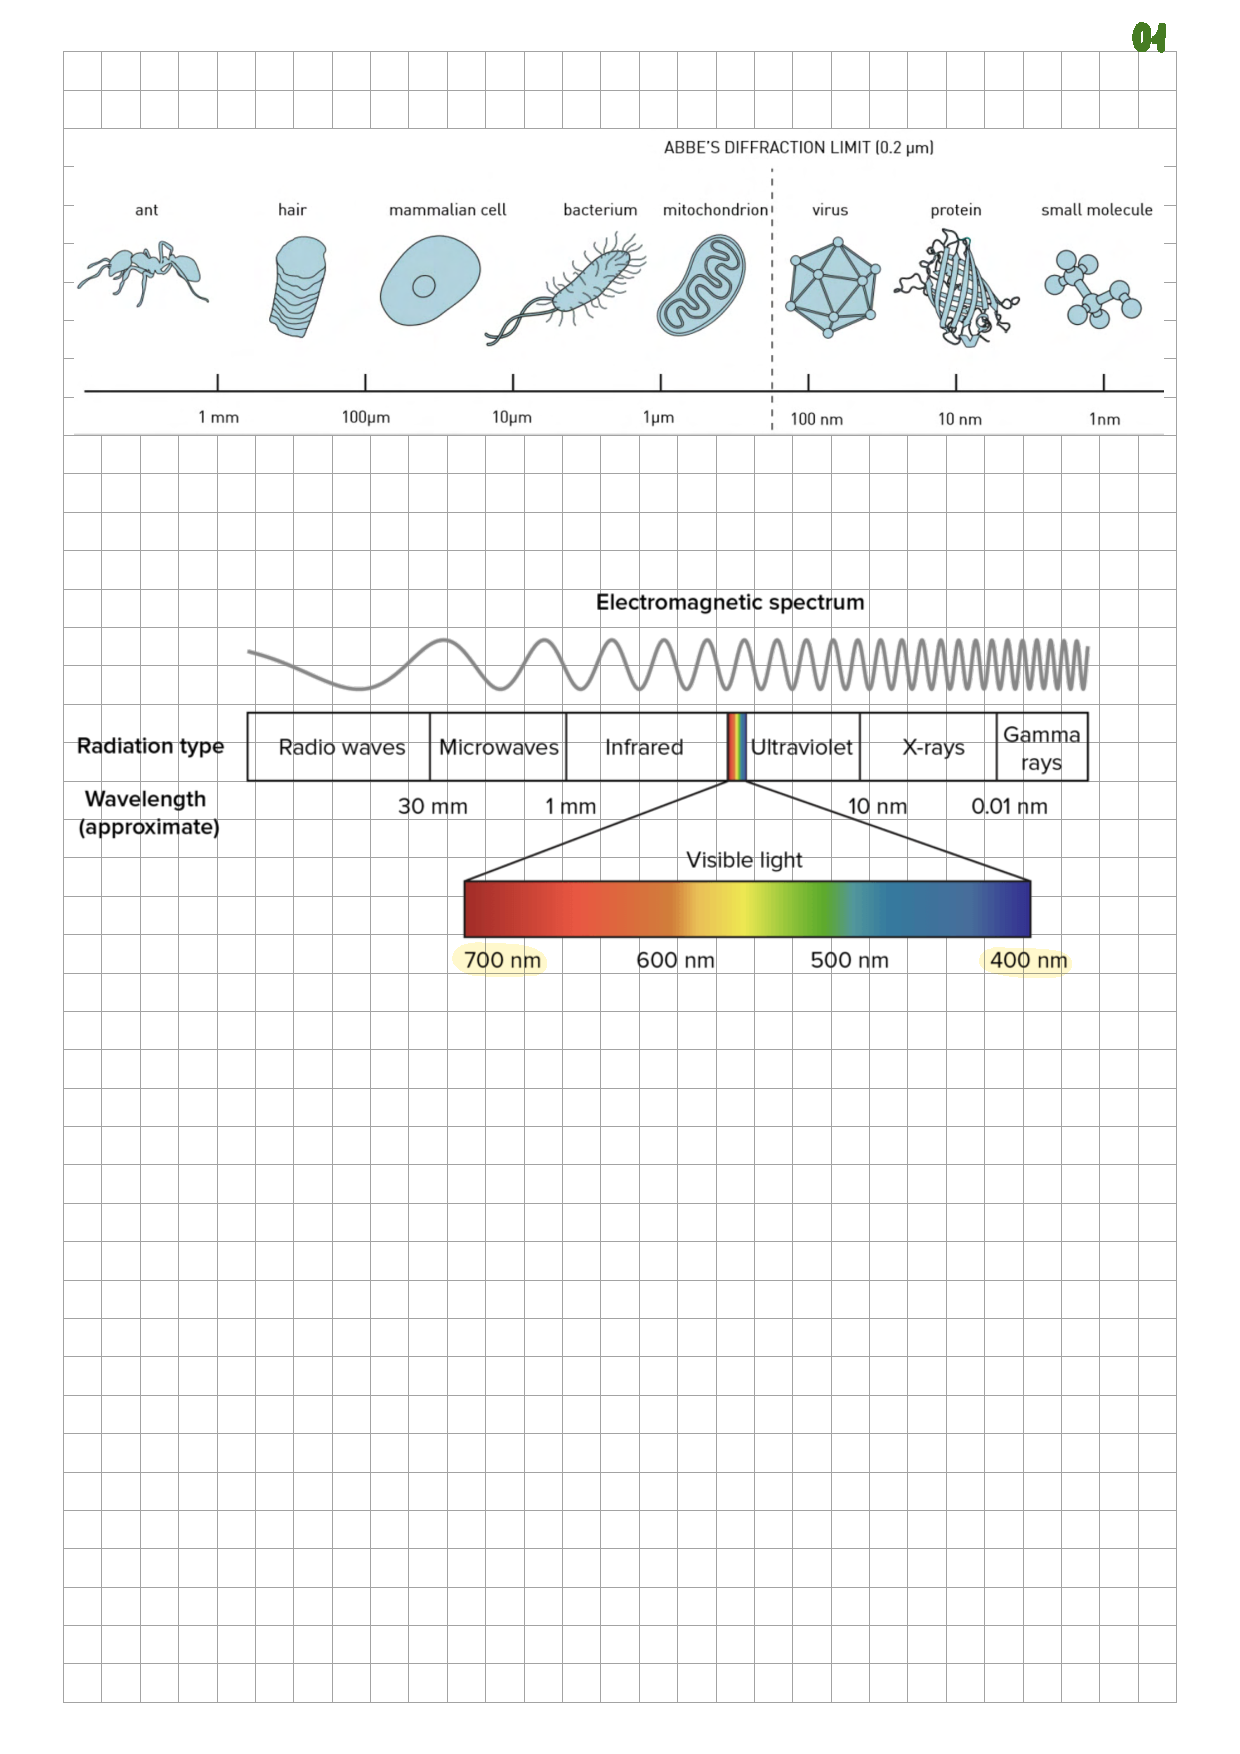
\includegraphics[width=0.5\textwidth]{pics/01.png}
\caption{Diagramma di fase qualitativo del modello di Hopfield.}
\end{figure}

Per caratterizzare le fasi, si usano parametri d'ordine come la sovrapposizione con una memoria $m^\mu$  e l'overlap tra repliche $q$:

\begin{align}
    m^\mu &= \frac{1}{N}\sum_i S_i \xi_i^\mu \\ 
    q &= \frac{1}{N}\sum_i S_i^{(1)}S_i^{(2)}
\end{align}

\begin{itemize}
\item \textbf{Fase Paramagnetica (P):} Ad alta temperatura, l'agitazione termica domina e gli spin sono orientati casualmente. Non c'è correlazione né con le memorie ($m=0$) né tra configurazioni diverse ($q=0$).

\item \textbf{Fase di Recupero (R - Retrieval):} A bassa temperatura e per un basso carico di rete ($\alpha < \alpha_c$), il sistema può recuperare le memorie. In questa fase, esistono stati termodinamicamente stabili in cui la sovrapposizione con una delle memorie è non nulla ($m \neq 0$). Il valore critico del carico a $T=0$ è $\alpha_c \approx 0.138$. Una rete di $N$ neuroni può memorizzare in modo affidabile al massimo circa il 14\% di $N$ pattern.

\item \textbf{Fase di Spin Glass (S):} Se il carico della rete supera la soglia critica ($\alpha > \alpha_c$), il sistema entra in una fase di spin glass. La sovrapposizione con le memorie è nulla ($m=0$), ma l'overlap tra repliche è non nullo ($q \neq 0$). Il paesaggio energetico diventa estremamente complesso, con un numero esponenziale di minimi locali ("stati spuri") che non corrispondono a nessuna delle memorie originali. La dinamica si blocca in questi stati spuri e il recupero fallisce.
\end{itemize}

\section{Problemi di Soddisfacimento di Vincoli (CSP)}

Un'altra area in cui le tecniche della meccanica statistica dei sistemi disordinati si sono rivelate fondamentali è lo studio dei \textbf{Constraint Satisfaction Problems} (CSP) in computer science. 

Un CSP è un problema di ottimizzazione combinatoria in cui si deve trovare una configurazione di variabili discrete che soddisfi un insieme di vincoli.  Consideriamo un sistema con:
\begin{itemize}
    \item $N$ variabili binarie, $S_i \in \{-1, 1\}$. 
    \item $M$ vincoli (o clausole). 
\end{itemize}

La difficoltà del problema è tipicamente misurata dal rapporto $\alpha = M/N$, ovvero il numero medio di vincoli per variabile. All'aumentare di $\alpha$, ci si aspetta una transizione da un regime in cui il problema è facilmente \textbf{soddisfacibile} (SAT) a uno in cui è \textbf{insoddisfacibile} (UNSAT). Nel limite termodinamico ($N \rightarrow \infty$), questa transizione diventa una \textbf{transizione di fase netta} (sharp transition), dove la probabilità che un'istanza random sia soddisfacibile passa da 1 a 0 in un punto critico $\alpha_s$. 

\begin{figure}[h!]
\centering
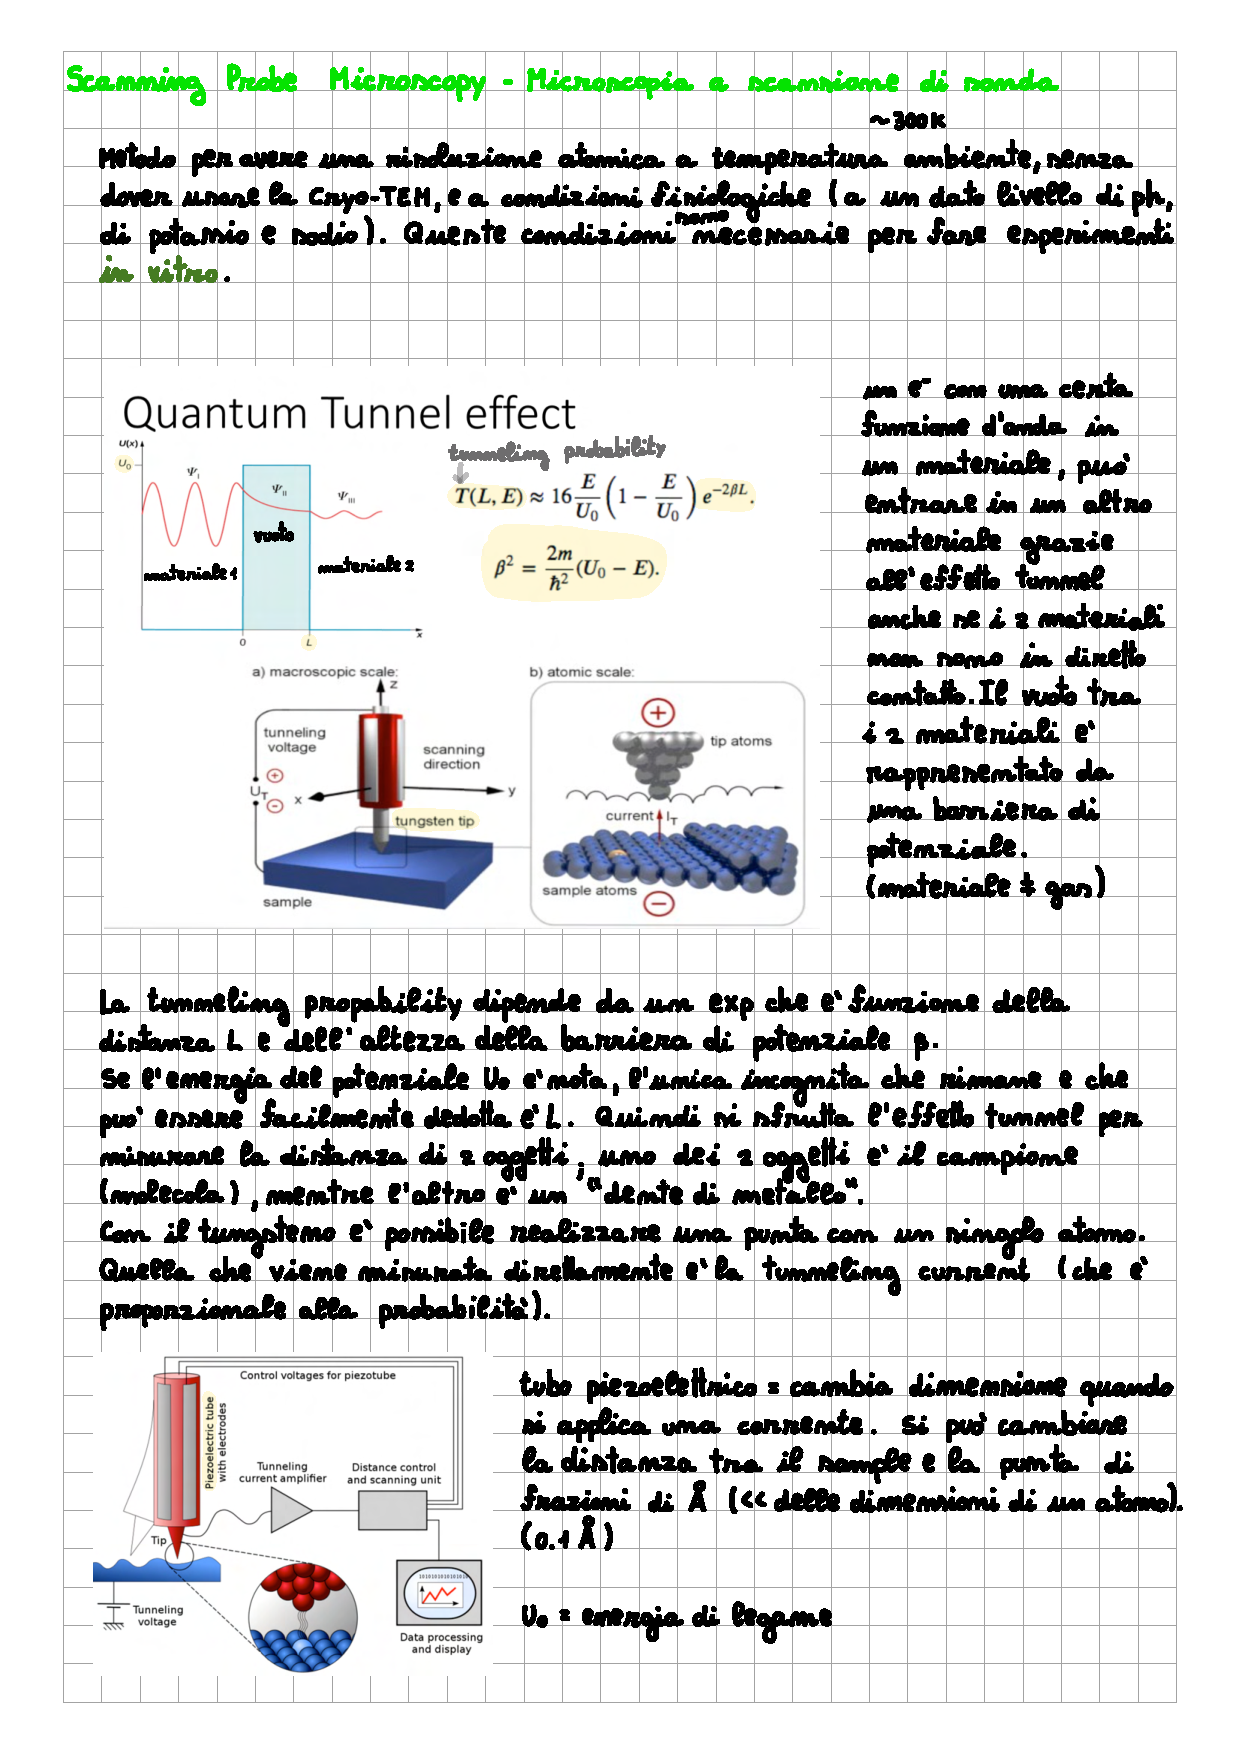
\includegraphics[width=0.5\textwidth]{pics/02.png}
\caption{Transizione di fase SAT/UNSAT.}
\end{figure}

Tuttavia, l'analisi ha rivelato una struttura più complessa. Per molti problemi, esiste una regione intermedia \textbf{SAT-HARD}, dove le soluzioni esistono ma sono estremamente difficili da trovare per gli algoritmi di ricerca locale. Gli algoritmi tipicamente riescono a trovare soluzioni fino a una soglia $\alpha_{d} < \alpha_s$, ma falliscono nella regione $[\alpha_{d}, \alpha_s]$. La fisica statistica ha fornito una spiegazione per questo fenomeno, collegandolo a un cambiamento nella struttura dello spazio delle soluzioni. 



\subsection{Il problema XORSAT}

Un problema apparentemente semplice che mostra questa struttura complessa è XOR-SAT. 
In termini di computer science, il problema è definito come segue:
\begin{itemize}
    \item $N$ variabili booleane $x_i \in \{\text{True, False}\}$ (o $\{0, 1\}$). 
    \item $M$ clausole, ognuna delle quali coinvolge 3 variabili scelte a caso $(i, j, k)$. 
    \item Ogni clausola impone un vincolo di \textbf{OR esclusivo (XOR)}: 
    $x_i \oplus x_j \oplus x_k = c_a$, dove $c_a$ è 0 o 1.
\end{itemize}
Se le variabili sono in $\{0, 1\}$, il vincolo si scrive come $(x_i + x_j + x_k) \pmod 2 = c_a$. 

Si tratta quindi di risolvere un sistema di $M$ equazioni lineari modulo 2 in $N$ incognite. Questo problema può essere risolto in tempo polinomiale (cubico, $O(N^3)$) con l'eliminazione gaussiana, che è un algoritmo globale. 
Tuttavia, gli algoritmi \emph{locali}, che usano solo informazioni locali, falliscono nel trovare soluzioni nella fase HARD. 

\subsubsection{Mappatura su un Modello di Spin}

Per studiare questo problema con la meccanica statistica, mappiamo le variabili booleane $x_i$ su variabili di spin $S_i$ tramite la trasformazione $S_i = (-1)^{x_i}$.  

Con questa mappatura, il prodotto di tre spin è legato alla somma delle variabili booleane:
\begin{equation}
  S_i S_j S_k =  (-1)^{x_i + x_j + x_k}   
\end{equation}


Per semplicità, consideriamo il caso in cui tutte le clausole devono essere soddisfatte con risultato 0, cioè $(x_i + x_j + x_k) \pmod 2 = 0$. 

\noindent Questo corrisponde a richiedere $S_i S_j S_k = 1$ per ogni clausola $(i,j,k)$

\noindent Una configurazione è una soluzione se soddisfa tutti gli $M$ vincoli:  $\sum_{(i,j,k)} S_i S_j S_k = M$.

Possiamo definire un'Hamiltoniana tale che il suo stato fondamentale (energia minima) corrisponda alle soluzioni del problema: 

\begin{equation}
H = M - \sum_{(i,j,k)} S_i S_j S_k
\end{equation}

Lo stato fondamentale ha energia $H=0$ e si raggiunge quando tutti i vincoli sono soddisfatti. Il disordine in questo modello non risiede negli accoppiamenti (che sono tutti uguali a -1), ma nella struttura del \textbf{grafo} di interazione, che è random poiché le triplette $(i,j,k)$ sono scelte a caso. 

\subsubsection{La Transizione di Fase e la Struttura delle Soluzioni}

Un calcolo semplice suggerisce che il numero di soluzioni dovrebbe essere $2^{N-M}$, poiché ogni equazione lineare indipendente dimezza lo spazio delle soluzioni. 

L'entropia (il logaritmo del numero di soluzioni) per spin sarebbe 
\begin{equation}
   S = \frac{1}{N} \log_2(2^{N-M}) = (1-\alpha)\log_2(1) 
\end{equation}

implicando che le soluzioni scompaiano solo per $\alpha_s = 1$. 

Tuttavia, sperimentalmente e teoricamente si trova che la soglia di soddisfacibilità è $\alpha_s \approx 0.918$. 
La discrepanza nasce dal fatto che il calcolo precedente assume che tutti i vincoli siano linearmente indipendenti, il che cessa di essere vero quando iniziano a formarsi dipendenze lineari. 
Ad un certo punto, si forma un sottoinsieme di variabili, chiamato \textbf{core}, che riceve un numero di vincoli così alto che diventa localmente insoddisfacibile, rendendo l'intero problema UNSAT anche se $\alpha < 1$. 

La transizione verso la fase HARD a $\alpha_d < \alpha_s$ è spiegata da un cambiamento topologico nello spazio delle soluzioni. 
\begin{itemize}
    \item \textbf{Fase EASY-SAT ($\alpha < \alpha_d$)}: Lo spazio delle soluzioni è un unico grande "cluster" connesso. È facile muoversi da una soluzione all'altra con piccole modifiche, e gli algoritmi locali possono esplorare questo spazio in modo efficiente. 
    
    \item \textbf{Fase HARD-SAT ($\alpha_d < \alpha < \alpha_s$)}: Lo spazio delle soluzioni, pur contenendo ancora un numero esponenziale di configurazioni, si frammenta in molti cluster piccoli e isolati. Si verifica una \textbf{rottura di ergodicità}. Questa clusterizzazione crea barriere energetiche che intrappolano gli algoritmi di ricerca locale in minimi locali di energia che non sono soluzioni, impedendo loro di raggiungere le vere soluzioni a energia zero. 
\end{itemize}

Questa transizione topologica, invisibile a livello dell'entropia totale (che rimane una funzione regolare di $\alpha$), è il vero ostacolo per gli algoritmi. 


\begin{figure}[h!]
\centering
\includegraphics[width=0.8\textwidth]{pics/03.png}
\caption{Rappresentazione del cambiamento topologico nello spazio delle soluzioni.}
\end{figure}


